\documentclass[landscape,final,a0paper,12pt]{baposter}

\usepackage{graphicx}
\usepackage{url}
\usepackage{multicol}
\usepackage{enumitem}
\usepackage{bm}
\usepackage{relsize}
\usepackage{multirow}
\usepackage{rotating}

%\setlength{\columnsep}{1.5em}
%\setlength{\columnseprule}{0mm}

\graphicspath{{images/}{./images/}}


\definecolor{darkblue}{HTML}{0000FF}
\definecolor{lightblue}{HTML}{00AAAA}
\definecolor{lightestblue}{HTML}{00FFFF}

\hyphenation{resolution occlusions}

\newcommand{\compresslist}{%
\setlength{\itemsep}{1pt}%
\setlength{\parskip}{0pt}%  
\setlength{\parsep}{0pt}%
}

\begin{document}

\begin{poster}
{
	grid = false,
	columns=3,
	bgColorOne = lightestblue,
	borderColor = lightblue,
	headerColorOne = white,
	headerFontColor = black,
	boxColorOne = white,
	textborder = rounded,
	eyecatcher = true,
	headerborder = closed,
	headerheight = 0.1\textheight,
	headershape = smallrounded,
	headershade = plain,
	headerfont =  \Large\bf\textsc,
	textfont = {\setlength{\parindent}{1.5em}},
	boxshade = plain,
	background = plain,
	linewidth = 2pt
}
{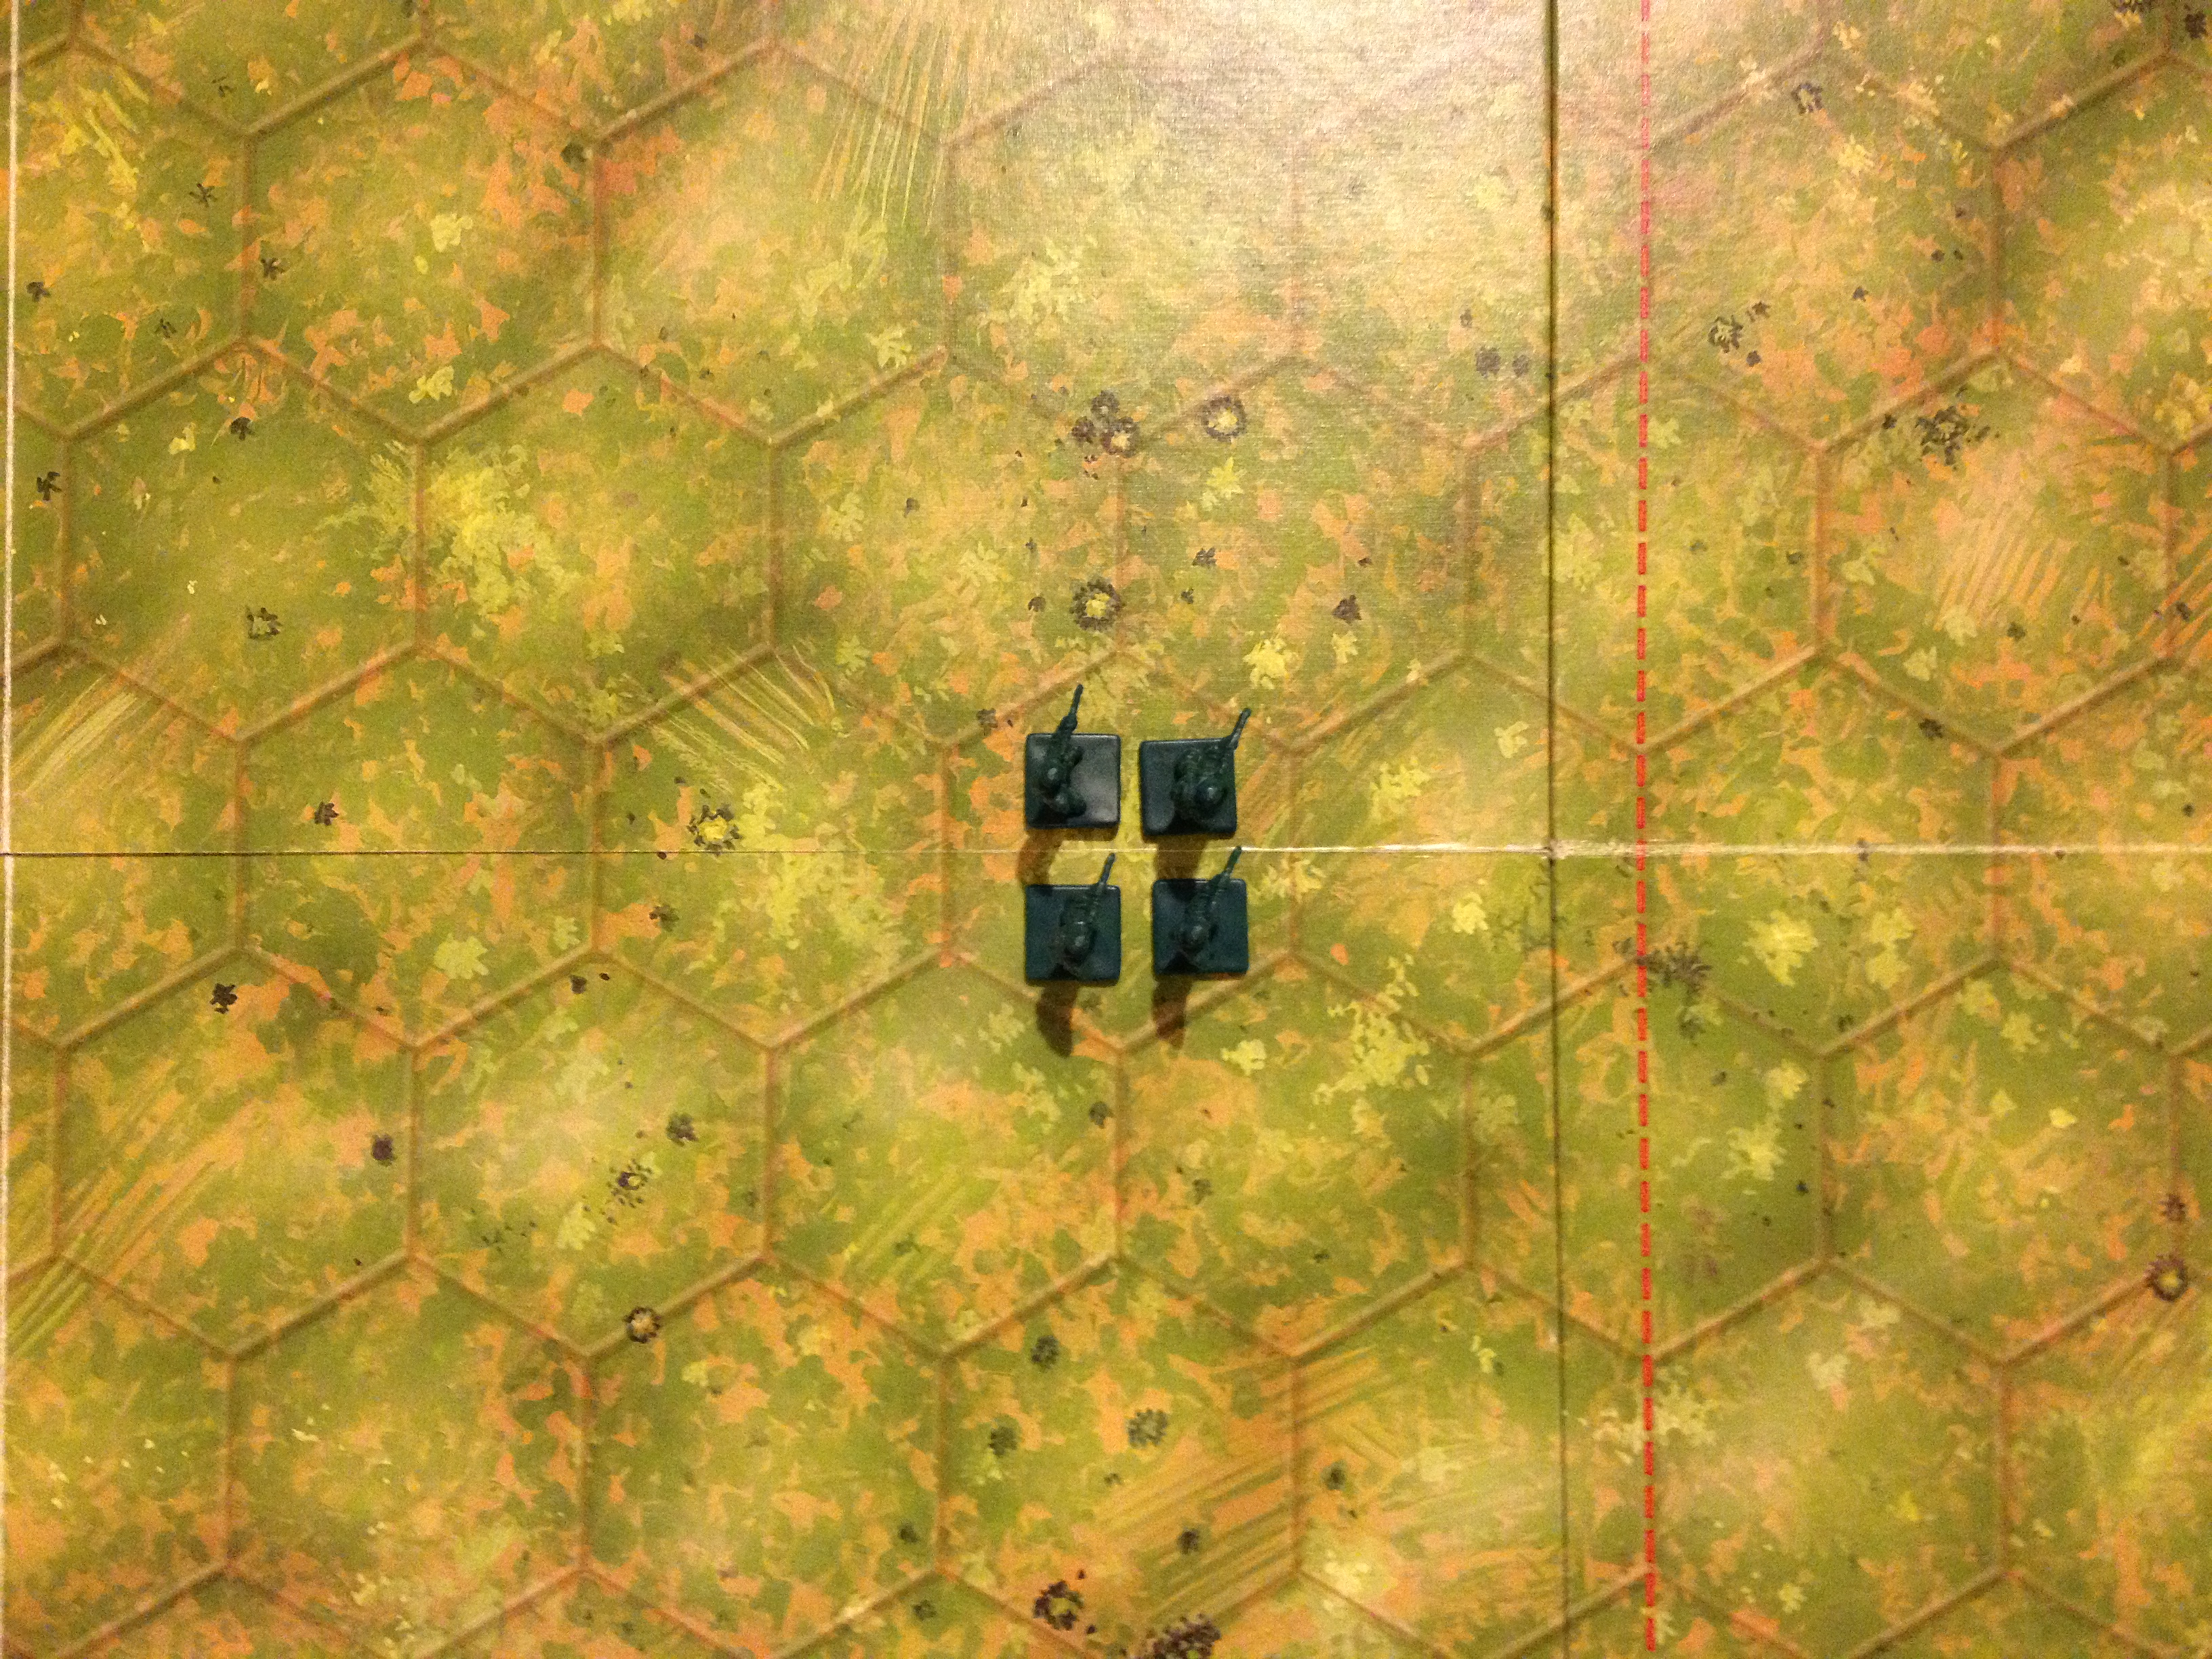
\includegraphics[height=6em]{./images/board_1}}
{\bf\textsc{Desert Fox: a Simple Wargame AI}\vspace{0.5em}}
{\textsc{Parker Michaelson}}
{
\includegraphics[height=6em]{./images/logo}}

\headerbox{Introduction}{name=intro, column=0, row=0}
{
Playing wargames, ranging from classics like Chess to Go to modern consumer games like Total War, presents a historically interesting problem for AI researchers.
Much progress has been made on the front of playing Chess and similar games with small search spaces and simple heuristics by using traditional search techniques.
Games with large search spaces which lack good heuristics, like Go, however, have presented a major challenge for such techniques.
Here we demonstrate the method of the {\it Monte Carlo Tree Search} for playing a simple game derived from the commercial game Memoir '44 called Desert Fox which, like Go, possesses a large search space and lacks effective heuristics.
}

\headerbox{General Strategy}{name=strategy, below=intro}
{
Desert Fox possesses a large search space compared to other games due to its simple, unrestrictive rules and large playing field.
On any given turn, a player may issue up to three orders to friendly units.
Orders may be to move to an adjacent tile, to fight an enemy unit on an adjacent tile, or to do nothing.
Play consists of alternating turns between the ``red'' and ``blu'' players until one of the players kills three enemy units.
This player wins the game regardless of the other player's score.
The board on which play occurs is rectangular in shape and consists of hexagons.
The board may be of any size so long as its width and height are odd.
Each player is assigned enough units to span the width of the board.
These units are placed at either length of the board.

\vspace{0.3cm}

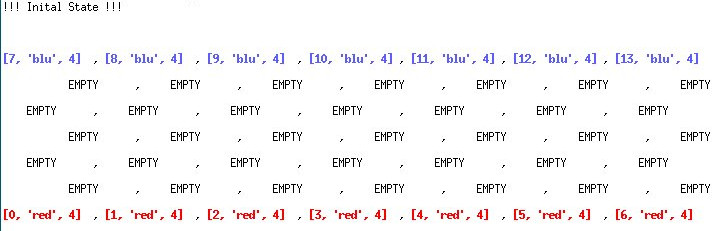
\includegraphics[width=0.9\colwidth]{./images/virtualboard_3.png}

\vspace{0.3cm}

The combination of many units and few restrictions leads to a swiftly growing combinatoric problem with an unreasonable size for a traditional unguided search.
Furthermore, a lack of good heuristics prevents both the implementation of a rule based player and the use of guided search techniques.
This project works around traditional limitations by using the Monte Carlo Tree Search (MCTS), which uses a large sampling of child states to find a close-to-optimal action for a given parent state.

% Annotate the algorithm.
}

\headerbox{Results}{name=results, column=1, row=0}
{
To test the strength of the MCTS algorithm, a series of experiments was performed in which the algorithm played against against a control player making moves entirely at random.
The experimental parameters varied in the experiments were the size of the board, ranging from 3x3 to 7x7, and the time budget allocated to computing a single order, ranging from 1 millisecond to 10 seconds.
Three hundred experiments were conducted at each data point.
The graph below plots the number of games from this sample won by the AI player at each point.

\vspace{0.3cm}

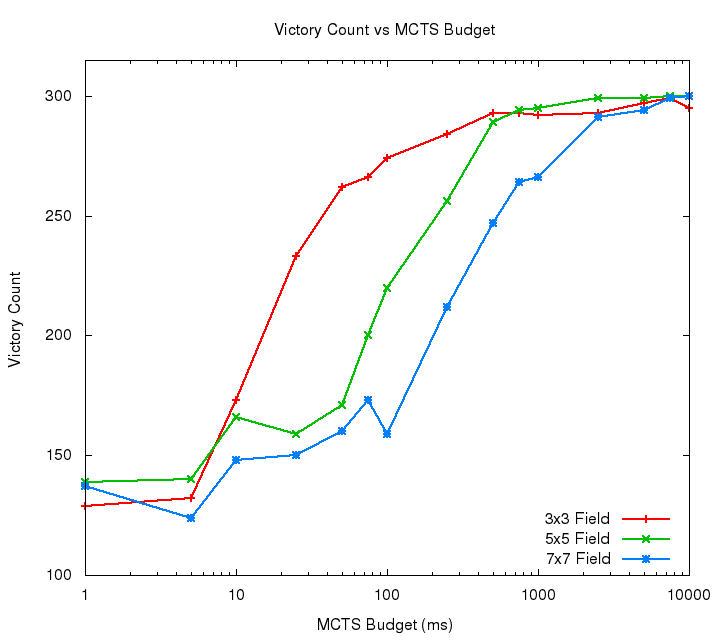
\includegraphics[width=0.9\colwidth]{./images/lineplot/lineplot}

\vspace{0.3cm}

A strong positive correlation is noted between the budget afforded to the MCTS algorithm and the number of games won by the AI player.
The number of wins by the AI player increased to almost 100\% of the sample when 10 seconds were allocated per decision.
This effect is a direct result of the MCTS algorithm having more time to sample potential moves, improving its chances of finding the best move.

The positive correlation between board size and win rate was unexpected.
That is to say that the MCTS algorithm consistently performed better on the larger of any two boards.
At first seems counterintuitive, but examining the properties afforded the random player reveals a simple explanation.
On smaller boards with few decisions to be made, the probability of the random player picking optimal or close-to-optimal moves is significantly increased by virtue of the small population from which moves are sampled.
In other words, a small board means that there are fewer ways to make a ``wrong'' decision.
This improved the performance of the control player relative to the AI player.
}

\headerbox{Conclusion}{name=conclusion, column=2, row=0}
{
Based on the performance of MCTS algorithm in the experimental trials, we see that its main strength comes about when faced with a large problem space.
Furthermore, we see that the performance of MCTS improves steadily with the increase of the computation budget.
In smaller search spaces or with low computation budgets, the performance of MCTS tends to be equal to or worse than an algorithm picking moves at random while also being much slower than the random player.

% Fix this later.
This logic extends to rule-based AI systems such as reflex agents.

It is reasonable to speculate that promising future work in this area could focus either on increasing the strength of an MCTS algorithm by increasing the number of simulations that can be performed within the computational budget, or by adding a learning system, such as Q-Learning, as a heuristic to better focus the attention of an MCTS algorithm on promising actions.
}

\headerbox{References}{name=references, column=2, below=conclusion}
{
% Fix ref issue.
\begin{thebibliography}{9}

%  \bibitem{amato10}
%  High-level Reinforcement Learning in Strategy Games. Christopher Amato and Guy Shanai. {\it Proc. of 9\textsuperscript{th} Int. Conf. on Autonomous Agents and Multiagent Systems (AAMAS 2010).}

  \bibitem{brown09}
  A Survey of Mente Carlo Tree Search Methods. Browne, Powley, {\it et. al.}. {\it IEEE Transactions of Computational Intelligence and AI in Games, Vol. 4, No. 1, MARCH 2012.}

\end{thebibliography}
}

\headerbox{Source Code}{name=source, column=2, below=references}
{
The source code is available as a Git repository at:

\indent{    } \url{github.com/pcm2718/psychic-pikeman.git}
}

\end{poster}

\end{document}
